\documentclass{article}

\usepackage[italian]{babel}
\usepackage[margin=2cm, footskip=5mm]{geometry}
% questi package non sono necessari in lualatex; ref https://tex.stackexchange.com/a/413046
% \usepackage[utf8]{inputenc}
% \usepackage[T1]{fontenc}
\usepackage{enumitem}
\usepackage{hyperref}
\usepackage{titlesec}
\usepackage{soulutf8}
\usepackage{contour}
\usepackage{float}
\usepackage{graphicx}
\usepackage{fancyhdr}
\usepackage{longtable}
\usepackage[table]{xcolor}
\usepackage{titling}
\usepackage{lastpage}
\usepackage{ifthen}
\usepackage{calc}
\usepackage{minted}
\usepackage{pgfgantt}
\usepackage{subfiles}

\newlength{\imgwidth}

\newcommand\scalegraphics[1]{%
    \settowidth{\imgwidth}{\includegraphics{#1}}%
    \setlength{\imgwidth}{\minof{\imgwidth}{\textwidth}}%
    \includegraphics[width=\imgwidth]{#1}%
}

% XXX definizione dei percorsi in cui cercare immagini
\graphicspath{ {./}
    {./img/}
}

% esempio di utilizzo: \appendToGraphicspath{./img/} (un comando diverso per ogni path da includere)
% N.B.: ci DEVE essere un forward slash alla fine del path, a indicare che è una cartella.
\makeatletter
\newcommand\appendToGraphicspath[1]{%
  \g@addto@macro\Ginput@path{{#1}}%
}
\makeatother

% setup della sottolineatura
\setuldepth{Flat}
\contourlength{0.8pt}

\newcommand{\uline}[1]{%
  \ul{{\phantom{#1}}}%
  \llap{\contour{white}{#1}}%
}

% setup dei link
\hypersetup{
  colorlinks=true, % set true if you want colored links
  linktoc=all,     % set to all if you want both sections and subsections linked
  linkcolor=black, % choose some color if you want links to stand out
}

% setup di header e footer
\pagestyle{fancy}

\fancyhf{}
\fancyhead[L]{\includegraphics[width=1cm]{logo.png}}
\fancyhead[R]{\thetitle}
\fancyfoot[R]{\thepage\ di~\pageref{LastPage}}

\fancypagestyle{nopage}{%
  \fancyfoot{}%
}

\setlength{\headheight}{1.2cm}

% setup forma \paragraph e \subparagraph
\titleformat{\paragraph}[hang]{\normalfont\normalsize\bfseries}{\theparagraph}{1em}{}
\titleformat{\subparagraph}[hang]{\normalfont\normalsize\bfseries}{\thesubparagraph}{1em}{}

% setup profondità indice di default
\setcounter{secnumdepth}{5}
\setcounter{tocdepth}{5}

% shortcut per i placeholder
\newcommand{\plchold}[1]{\textit{\{#1\}}} % chktex 20

% hook per lo script che genera il glossario
\newcommand{\glossario}[1]{\underline{#1}\textsubscript{g}}

% definizione dei comandi \uso e \stato
\makeatletter
\newcommand{\setUso}[1]{%
  \newcommand{\@uso}{#1}%
}
\newcommand{\uso}{\@uso}

\newcommand{\setStato}[1]{%
  \newcommand{\@stato}{#1}%
}
\newcommand{\stato}{\@stato}

\newcommand{\setVersione}[1]{%
  \newcommand{\@versione}{#1}%
}
\newcommand{\versione}{\@versione}

\newcommand{\setResponsabile}[1]{%
  \newcommand{\@responsabile}{#1}%
}
\newcommand{\responsabile}{\@responsabile}

\newcommand{\setRedattori}[1]{%
  \newcommand{\@redattori}{#1}%
}
\newcommand{\redattori}{\@redattori}

\newcommand{\setVerificatori}[1]{%
  \newcommand{\@verificatori}{#1}%
}
\newcommand{\verificatori}{\@verificatori}

\newcommand{\setDescrizione}[1]{%
  \newcommand{\@descrizione}{#1}%
}
\newcommand{\descrizione}{\@descrizione}

\newcommand{\setModifiche}[1]{%
  \newcommand{\@modifiche}{#1}%
}

\newcommand{\modifiche}{\@modifiche}

\makeatother

% setup delle description
\setlist[description,1]{font=$\bullet$\hspace{1.5mm}, labelwidth=* leftmargin=*,labelindent=12.5mm}
\setlist[description,2]{font=$\bullet$\hspace{1.5mm}, leftmargin=*,labelindent=12.5mm}

\appendToGraphicspath{../../commons/img/}

\title{Verbale --- 16/12/2019}

\setVersione{\plchold{versione}}
\setResponsabile{Alessandro Rizzo}
\setRedattori{Riccardo Agatea}
\setVerificatori{}
\setStato{WIP}
\setUso{Esterno}
\setDescrizione{Verbale dell'incontro di GruppOne del 16/12/2019}
\setModifiche{}

\begin{document}

\thispagestyle{empty}
\pagenumbering{gobble}

\begin{center}

  \includegraphics[width=8.5cm]{\commons/img/logo.png}\\
  {\Large GruppOne - progetto "Stalker"}\\
  \vspace{1.5cm}

  {\Huge \thetitle}
  \vspace{1.5cm}

  \begin{table}[H]
    \centering

    \begin{tabular}{r|l}
      \textbf{Versione}     & \versione              \\
      \textbf{Approvazione} & \responsabile          \\
      \textbf{Redazione}    & \redattori             \\
      \textbf{Verifica}     & \verificatori          \\
      \textbf{Stato}        & \stato                 \\
      \textbf{Uso}          & \uso                   \\
      \textbf{Destinato a}  & Imola Informatica      \\
                            & GruppOne               \\
                            & Prof. Tullio Vardanega \\
                            & Prof. Riccardo Cardin  \\
    \end{tabular}
  \end{table}

  \vspace{3cm}
  \textbf{Descrizione}\\
  \descrizione\\
  \vfill
  \verb|gruppone.swe@gmail.com|
\end{center}

\newpage
\thispagestyle{nopage}

\section*{Registro delle modifiche}
\label{sec:registro_delle_modifiche}

\begin{table}[H]
  \label{tab:registro_delle_modifiche}

  \centering
  \rowcolors{2}{lightgray}{white!80!lightgray!100}

  \begin{longtable}[c]{c c c c l}
    \rowcolor{darkgray!90!}\color{white}{\textbf{Versione}} & \color{white}{\textbf{Data}} & \color{white}{\textbf{Nominativo}} & \color{white}{\textbf{Ruolo}} & \color{white}{\textbf{Descrizione}} \\\endhead
    \modifiche
  \end{longtable}
\end{table}

% section registro_delle_modifiche (end)
\newpage

\thispagestyle{nopage}
\pagenumbering{roman}
\tableofcontents

\newpage

\pagenumbering{arabic}

\section{Ordine del giorno}%
\label{sec:ordine_del_giorno}

\begin{itemize}
  \item GDPR
  \item Server LDAP
  \item Varie ed eventuali
\end{itemize}
\section{GDPR}%
\label{sec:gdpr}
Il sistema deve rispettare la normativa GDPR\@.
In fase di progettazione architetturale, dovremo scegliere accuratamente le minime informazioni relative agli utenti necessarie per la registrazione di utenti e organizzazioni, e per il tracking.
Dovremo successivamente strutturare il database in modo che i dati siano separati (ad esempio, in un database relazionale devono essere in tabelle diverse), per evitare problemi di sicurezza.
Per verificare se l'architettura decisa rispetta la normativa, il proponente ha consigliato di utilizzare delle checklist facilmente reperibili on-line.
Abbiamo comunque rimandato la discussione al periodo successivo alla Revisione dei requisiti.
% sec:gdpr (end)
\section{Server LDAP}%
\label{sec:server_ldap}
Il sistema da sviluppare non deve necessariamente implementare un server LDAP, deve solo permettere alle organizzazioni di utilizzare il proprio per autenticare gli utenti.
D'altro canto, per la fase di test e collaudo ci sarà necessario avere a disposizione un server LDAP, che quindi dovremo implementare per lo meno parzialmente.
Inoltre, LDAP può essere utilizzato per l'autenticazione degli utenti di Stalker.
% sec:server_ldap (end)
\section{Varie ed eventuali}%
\label{sec:varie_ed_eventuali}
\subsection{Definizione dei luoghi}%
\label{sub:definizione_dei_luoghi}
La definizione dei luoghi deve essere di responsabilità delle organizzazioni, con dei limiti imposti.
I limiti sono necessari per evitare che un'organizzazione occupi uno spazio eccessivo nel server definendo molti luoghi, e al contempo per evitare che un'organizzazione monitori luoghi di cui non dovrebbe interessarsi (come luoghi pubblici o edifici privati non di sua proprietà).\par
È sufficiente che la definizione dei luoghi sia tramite approssimazioni a quadrilatero.
In fase di progettazione dovremo decidere (e documentare) il livello di approssimazione. Non è necessario che il tracking consideri l'altitudine.
% sub:definizione_dei_luoghi (end)
\subsection{Sicurezza}%
\label{sub:sicurezza}
Il database potrà essere non criptato, ma la scelta dovrà essere documentata e riportata all'utente.
% sub:sicurezza (end)
% sec:varie_ed_eventuali (end)
\end{document}
